\documentclass[twocolumn, 10pt]{jsarticle}
% pLaTeX/upLaTeX環境
\bibliographystyle{jIEEEtran}
\usepackage[top=15truemm,bottom=15truemm,left=10truemm,right=10truemm]{geometry}
\pagestyle{empty}
\usepackage[dvipdfmx]{graphicx}
\usepackage[dvipdfmx]{color}
\usepackage[dvipdfmx]{xcolor}
\usepackage{amsmath}
\usepackage{amssymb}
\usepackage{cite}
\usepackage{subcaption}
\usepackage{ascmac}
\usepackage[hyphens]{url}
\usepackage{booktabs}
\usepackage{array}
\usepackage{multirow}

\title{品質の高いソフトウェアの設計}
\author{23266025 大森俊弥}
\date{2026年3月20日}

\begin{document}
\maketitle

\section{はじめに}

企業でソフトウェアの開発に携わると，単一の機能の実現可能性以上に，現実の制約や将来的な拡張に耐えうる設計が求められる．したがって，アーキテクチャ設計の規則など，品質の優れたソフトウェアを実装するための具体的な設計思想は，実務に携わる際に重要である\cite{evans2003ddd,martin2017cleanarchitecture,fowler2003eaa}．しかし，実務上の制約を意識した設計の知見を学生の間に得られる機会は稀である．本稿では，ソフトブレーン株式会社における筆者の開発経験を基に，現場で役立つ設計思想をいくつか紹介する．なお，筆者が携わる製品は，社員のデータを共有することで業務を最適化するシステムである．システムには，ユーザに使い方を説明するためのヘルプ記事が整備されている．本稿の題材には，「自然言語による指示に応じた操作支援機能」，「ヘルプ記事に基づく質問応答チャット機能」の2つの新機能開発を取り上げる．前者ではフロントエンド（ユーザの画面側）における関数の責務と依存関係，後者ではバックエンド（サーバ側）における非同期処理とベクトル検索に着目する．さらに，これらを支えるコードレビューの観点についても述べる．チームにおける開発や，就職後の開発の参考となれば幸いである．

\section{フロントエンド設計の要点}
本章では，「自然言語による指示に応じた操作支援機能」を題材に，機能同士の関係に関する考え方を説明する．
\subsection{アーキテクチャの境界と依存性のルール}

フロントエンド設計では，保守と拡張を可能とするために，関心の異なる機能を分離することが重要である．目的の異なる処理を同一箇所で実装すれば，コードを変更した際の影響範囲は大きくなる．この課題に対して，Martin は機能を役割ごとに階層的に分離する Clean Architecture を提唱している\cite{martin2017cleanarchitecture}． 設計において，各機能が担う役割の範囲は責務と呼ばれる．責務を明確に分離することで，機能は特定の目的に専念できる．Clean Architecture により，機能を他の複数の機能から活用できる再利用性や，影響範囲の限定による変更容易性が向上する．

また，ある機能が他の機能を利用する関係は依存関係と呼ばれる．依存関係が無秩序に広がると，一部の変更が広範な不具合の原因となり得る．図\ref{fig:clean_architecture}に示すように，Clean Architecture では画面の制御や外部との通信を担うコードは中核となるロジックに依存してよい一方で，中核のロジックは画面の表示方法や通信手段に依存してはならない．

\begin{figure}[t]
    \centering
    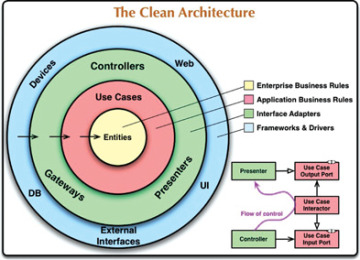
\includegraphics[width=0.9\linewidth]{clean_architecture.jpg}
    \caption{Clean Architecture における依存方向の概念図．}
    \label{fig:clean_architecture}
\end{figure}

\subsection{ユースケース層の独立}

責務と依存方向を明確にする方法は，アプリケーションの中核となるロジックを画面制御用の関数群から分離して実装することである．外部からの要求を実現する中核的な処理は，ユースケース（Application Business Rules）層と呼ばれる\cite{martin2017cleanarchitecture}．例えば操作指示に応じた支援機能では，社員一覧画面を開いている利用者が「画面に表示されている社員で 30 分の会議を設けたい」と自然言語で指示する場面を想定している．この指示に応じて，支援機能は表示されている社員の一覧を取得する関数を呼び出す．Vue.js の枠組みは，この関数を画面表示を制御する関数からディレクトリ単位で明確に分離することで，関数が取得機能に専念できる実装を実現している．

\subsection{インタフェースアダプタによる状態取得}
前節で述べたユースケース層の独立を実現するためには，画面や外部との入出力をユースケース層が直接扱わない構成にすることが重要である．
操作指示に応じた支援機能では，インタフェースアダプタ（Interface Adapters）層を導入することで，画面側の状態取得とバックエンド連携をユースケース層から分離し，変更影響を局所化した構造を実現できる．インタフェースアダプタ層は，ユースケース層と User Interface（UI）や外部のシステムとの間に位置する（図\ref{fig:clean_architecture}）．画面側で取得した状態をユースケース層が扱いやすい形式へ変換し，逆にユースケース層の出力を UI や外部システムが利用しやすい形式へ変換する責務を担う\cite{martin2017cleanarchitecture}．バックエンド側の処理が画面の状態へ直接依存すると，画面の小規模な変更が機能全体の破壊を招く可能性がある．状態取得とデータ変換をインタフェースアダプタ層に集約することで，画面側の変更による影響を最小化できる．

\section{バックエンド設計の要点}
本章では，「ヘルプ記事に基づく質問応答チャット機能」を題材に，非同期処理とベクトル検索の設計について述べる．
\subsection{非同期処理とジョブ管理}

前章で述べた責務や依存関係の整理は，バックエンド設計においても重要である．実運用では，システムの信頼性を担保するために，状態の変化を伴う処理を慎重に設計することや，処理の失敗を想定した堅牢な実装がより重要視される．


ヘルプ記事に基づく質問応答チャットは，Retrieval-Augmented Generation（RAG）によって実現される．実運用においてヘルプ記事は更新されるため，埋め込み生成から失敗時処理までの一連のジョブを頻繁に実行する必要がある．このような待ち時間の長い処理の高速化には，一般に Python の \texttt{asyncio} に代表される非同期処理系が有効である\cite{python_asyncio}．独立な非同期処理群の合流をコード上に明示することは，データベース更新のような状態を変化させる処理を安全に直列化することにも結び付く．
このとき，データベース設計では成功経路よりも失敗時の整合性維持が重要である．本番環境では失敗時に備えて，ファイルサイズに依存するタイムアウトおよび再試行の設計を行う．

\subsection{ユーザ体験を想定したRAG}

ヘルプ記事に基づく質問応答チャットをはじめ，RAG を応用したシステムではベクトル検索基盤の性能がユーザ体験に直結する．セマンティック類似度（Semantic Similarity）のみを用いた検索では，無関係な機能のヘルプ記事を参照し，誤った情報を提供する恐れがある．逆に現在表示中の画面に関する記事のみを検索対象とすることも，ユーザの質問意図から乖離した応答を提供する可能性がある．
この課題を解決するため，各記事 $i$ の内容を表すベクトル $v_i$，記事の目的や対象機能に関する要約ベクトル $s_i$ を加算したのち L2 正規化を行うことで，次式で示される新たな合成ベクトル $v'_i$ を算出する．
\begin{equation}
    v'_i = \frac{v_i + s_i}{\|v_i + s_i\|}
    \label{eq:vector_norm}
\end{equation}
この $v'_i$ によって記事を配置することで，ひとつのベクトル空間上で機能ごとに分離した配置に対して検索を実行できる．これにより，画面の状態を検索の制約としないまま，無関係な情報の参照を防ぐことができる．

\section{コードレビューの観点}

企業における開発では，開発者が行ったコードの変更は反映前に必ずレビューを受ける．レビューでは，個々のコード片の巧拙のみならず，これまで述べてきたように保守性と拡張性が重視される．責務の分離や依存方向のほかに，実務上特に重要なレビュー観点を表\ref{tb:review} に示す\cite{fowler2018refactoring,martin2017cleanarchitecture}．取得値が確定する実装や修正範囲を限定する工夫によって，複数の開発者が安全に修正し，障害時に迅速に復旧できる構造を維持できる．したがって，レビュワーとの議論は静的な品質保証ではなく，将来の運用と変更を見越した設計過程と捉えることができる．

\begin{table}[t]
    \centering
    \caption{現場で重視される主なレビュー観点}
    \label{tb:review}
    \begin{tabular}{>{\raggedright\arraybackslash}p{0.23\linewidth} >{\raggedright\arraybackslash}p{0.69\linewidth}}
        \toprule
        観点 & 主な確認内容 \\
        \midrule
        状態の真正性 & 取得値に未確定値が含まれないか\\
        冪等性 & 再試行や二重送信時に副作用が重複しないか \\
        障害時の挙動 & タイムアウト・例外・部分失敗時に整合性が確保されるか \\
        拡張容易性 & 画面追加や仕様変更時に修正範囲が局所化されるか \\
        コスト & 外部サービスの呼び出し量，ストレージ量，想定するキャッシュ占有量が妥当か \\
        \bottomrule
    \end{tabular}
\end{table}


\section{おわりに}

本稿では，新機能開発の事例を通して，企業の開発の現場における設計判断のポイントを整理した．フロントエンドでは，責務の分離と依存方向の整理によって高い保守性と拡張性を実現することが重要である．バックエンドでは，非同期処理や検索設計により運用時の堅牢性と利用体験を向上させることができる．本稿で述べた観点は特定の技術や機能に限らず，一般的なシステム開発に共通して応用可能である．将来の変更や運用も見据えた設計判断の参考としてほしい．

\bibliography{ref}
\end{document}